\documentclass[a4paper,11pt,parskip=never,DIV=8,chapterprefix=true,titlepage=true,twoside,twocolumn,open=any]{scrbook}
%\usepackage{mathptmx}% http://ctan.org/pkg/times
\usepackage{tgpagella}
%\usepackage[osf,sc]{mathpazo}% http://ctan.org/pkg/times
%\usepackage[sc]{mathpazo}% http://ctan.org/pkg/times
\linespread{1.05}
\setcounter{secnumdepth}{0}
\renewcommand*\sectfont{\normalcolor\bfseries}% removed \sffamily
%\setparsizes{1em}{0.25\baselineskip plus .25\baselineskip}{1em plus 1fil} 
\usepackage[T1]{fontenc}
\usepackage{textcomp} % provide euro and other symbols
\usepackage[labelformat=empty,font=small]{caption}
\usepackage{float}
\usepackage{caption}
\usepackage{amsmath}
\usepackage{amssymb}
\usepackage{lettrine}
\usepackage[export]{adjustbox}
\usepackage{graphicx}
\usepackage{xcolor}
\usepackage{booktabs}
\usepackage{enotez}
\usepackage[english]{babel}
\usepackage{blindtext}
\usepackage{lipsum}
\setlength{\columnsep}{.7cm}
\addtokomafont{section}{\normalsize}
\addtokomafont{subsection}{\normalsize}
\usepackage{balance}
\usepackage{makeidx}
%\usepackage{showframe}
%\usepackage[showframe]{geometry}
\usepackage{geometry}
\usepackage{enumitem}
\setitemize{noitemsep,topsep=0pt,parsep=0pt,partopsep=0pt}
\renewcommand\labelitemi{$\vcenter{\hbox{\tiny$\bullet$}}$}
\AfterCalculatingTypearea{\geometry{margin=2cm,top=3cm,bottom=3.5cm,bindingoffset=6mm}}
%\AfterCalculatingTypearea{\geometry{margin=2.5cm,top=5cm,bottom=5cm,bindingoffset=12mm,nofoot}}
\recalctypearea

%\usepackage[showframe]{geometry}
%\usepackage{geometry}
%\usepackage[%
%  a4, % <===============================================================
%  axes,cross,pdftex,center
%]{crop}

\DeclareInstance{enotez-list}{plain}{paragraph}{notes-sep=0pt}
\LettrineRealHeighttrue


\setenotez{
  reset=true,
  list-name=Endnotes,
  list-heading = \section*{#1},
  backref=true,
  list-style=plain
}

\DeclareInstance{enotez-list}{custom}{paragraph}
{
%format = \small ,
%format = \footnotesize ,
format = \scriptsize ,
%format = \tiny ,
notes-sep=0pt,
number = \textsuperscript{#1}
}
\let\footnote=\endnote
%\usepackage{biblatex}
%\usepackage{chapterbib}
\usepackage{import}
\usepackage{wrapfig}
\usepackage{upquote}
%\usepackage{bookmark}
%\usepackage{hyperref}
\usepackage{nicefrac}
\usepackage[noabbrev]{cleveref}
\usepackage[headsepline=true, autooneside=false]{scrlayer-scrpage}

\makeindex

\pagestyle{scrheadings}

\lohead{}
\cohead{}
\rohead{\leftmark}

\cofoot[]{}
\rofoot[\pagemark]{\pagemark}

\automark[section]{chapter}

\begin{document}

\begin{titlepage}
  \null\vfill
  \begin{center}
    \vskip 1em
    {%
      \usekomafont{title}{\Huge
        Christ Church Murgon% <- title
      \par}%
    }%
    \vskip 2em
    {%
      \usekomafont{subtitle}{%
        Celebrating 100 Years of Anglican Parish History% <- subtitle
      \par}%
    }%
    \vfill
    {%
      \usekomafont{author}{%
          Compiled By Marcia McIntosh% <- author
      \par}%
    }%
    \vskip 1.5em
    {\usekomafont{date}{\small \today \par}}%
  \end{center}
  \clearpage
  \thispagestyle{empty}
  \noindent\begin{minipage}[t]{\textwidth}
   {\small Printed By:\\T J Printing Group\\42 King St, Deception Bay QLD 4508\par \vskip 1.5em \today \par}
  \end{minipage}\par
  \vfill
  \noindent\begin{minipage}[b]{\textwidth}
  {\small This book was set with the help of {\KOMAScript} and {\LaTeX}}
  \end{minipage}\par

  \clearpage
  \thispagestyle{empty}
  \par\vspace*{.45\textheight}
  \noindent\begin{minipage}[b]{\textwidth}
  \begin{center}
    {\small In the spirit of reconciliation we acknowledge the Traditional Custodians
            of country throughout Australia and their connections to land, sea and community.
            We pay our respect to their elders past and present and extend that respect to all
            Aboriginal and Torres Strait Islander peoples today.}
  \end{center}
  \end{minipage}\par
\end{titlepage}
%\newpage
%\onecolumn
\frontmatter
{
\setcounter{tocdepth}{2}
\tableofcontents
}

%\newpage
%\cleardoublepage
\setchapterpreamble[o]{
\dictum[Psalm 56:3]{But when I am afraid,\linebreak I will put my trust in you.}}

%\chapter{Preface}
%
%\lettrine[lines=3]{C}{HRIST} Church Murgon, Anglican Church has stood proudly at the intersection of
%Taylor and Watt Streets since its construction in the latter months of 1919 though
%the history of Anglicanism in the region extends much further back than this date.
%A building is simply a physical structure to serve as a central bonding place of
%communal worship and of fellowship, mutual support and growth in faith for ``The Church''.
%The people who worship our Lord are God's Kingdom on earth.
%Resilient pioneering settlers of the Murgon district felt the need for a permanent place of
%worship.  Accordingly, the telling of the story of this building cannot be divorced from
%the events of the world during this historic period, and much less so from the story of
%the people who brought both it and the town of Murgon into being and who have served
%God and the community from the mid-1840s through the decades to where we are now.

%\newpage
%\cleardoublepage
\chapter{Foreword}
\blindtext
\blindtext
\blindtext

\twocolumn

\mainmatter
\setcounter{page}{1}

\setchapterpreamble[o]{
\dictum[Matthew 17:7]{And Jesus came and touched them, and said, Arise, and be not afraid.}}

\chapter{Introduction}
\lettrine[lines=3]{T}{HE} Murgon parish has grown from a dream in the minds of the 
European settlers who arrived after the opening of the railway in 1903 - timber getters, 
selectors, business people - who all developed the town of Murgon and surrounding 
districts. External factors - wars, depressions, weather conditions, advent of personal 
ownership of the motor car, and changing societal responses to organised religious 
observance � have influenced the role of the Murgon's Christ Church Anglican Church 
in the Barambah Parish. 

Murgon is a new town in comparison with its neighbours, Gayndah and Nanango. Murgon 
town established itself around the railway station. The town and surrounding farms 
were excised from \emph{Barambah}, \emph{Boonara} and \emph{Manumbar} pastoral stations. 
Cherbourg Aboriginal Community was reserved out of \emph{Barambah} and is part of 
the Barambah Parish. The uptake of land selections and town allotments was steady.

\begin{figure}
\begin{center}
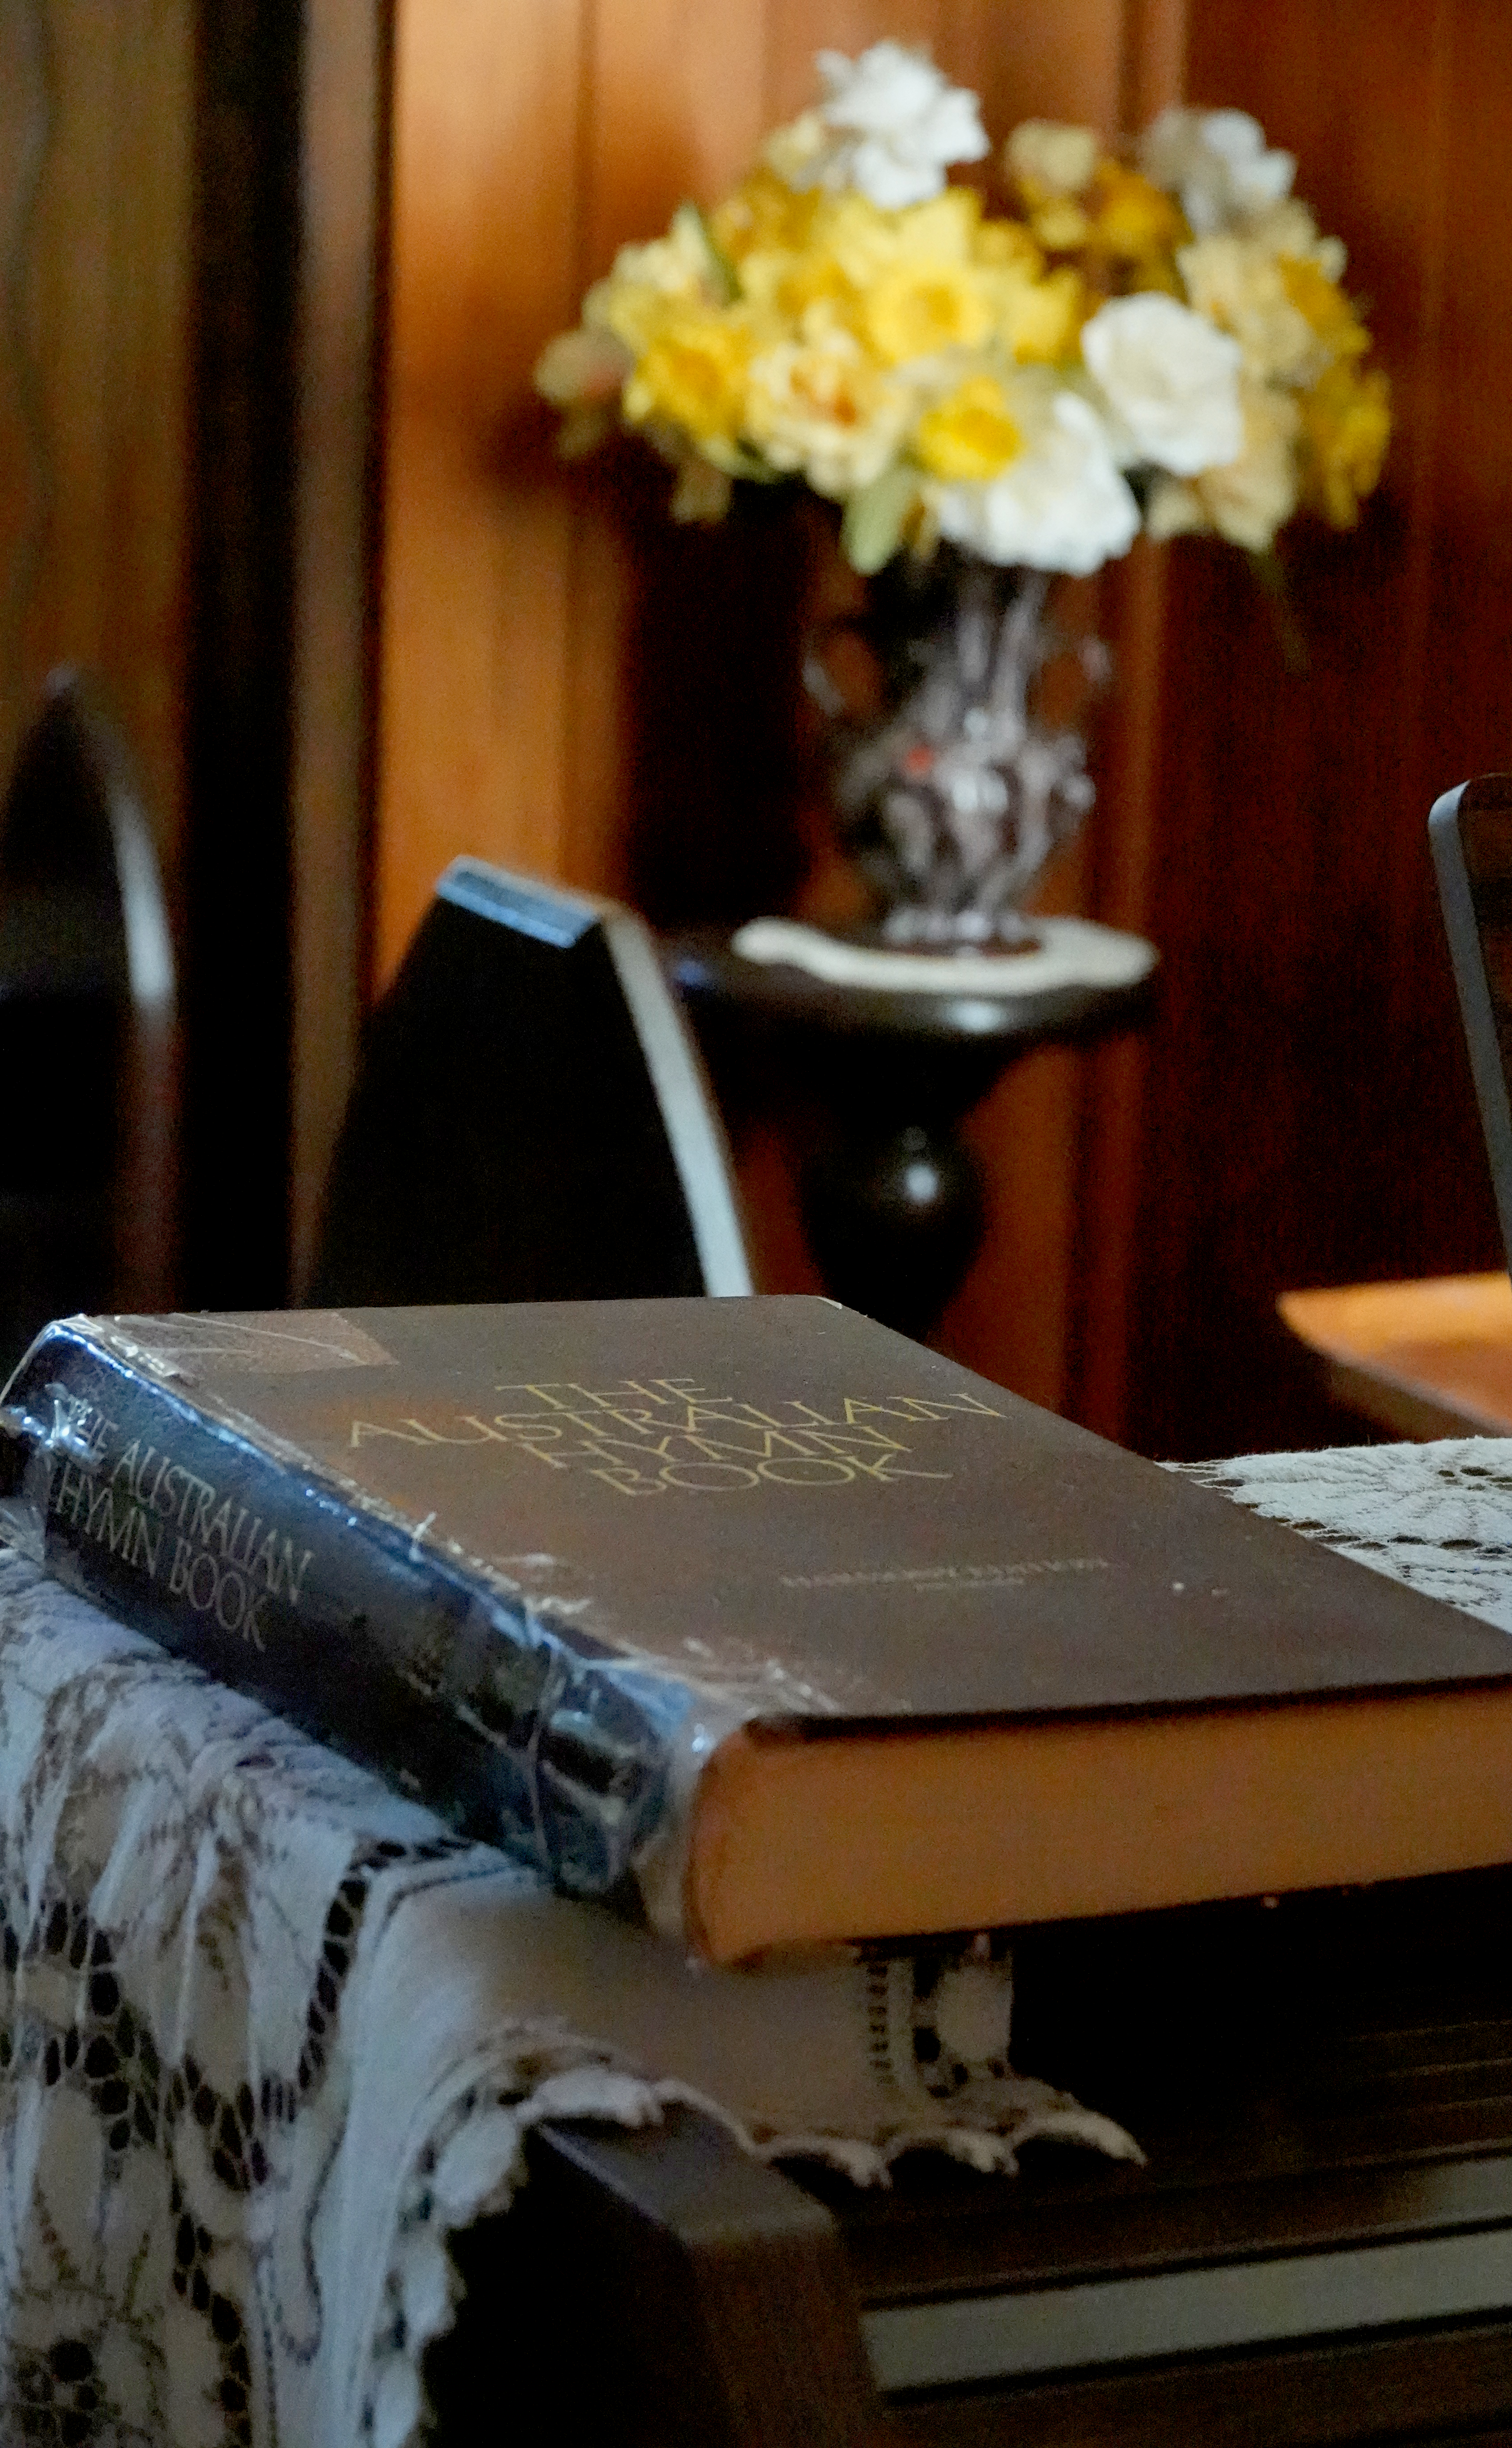
\includegraphics[width=1.\linewidth,center]{../images/theAustralianHymnBook.jpg}
\end{center}
\end{figure}

The South Burnett has been a highly productive agricultural region since the arrival 
of European settlers. Group Settlements were organised of young men from northern 
New South Wales, the Fassifern and Lockyer districts and Brisbane before World War I 
seeking opportunities in the new settlements. Extraction of the pine timber on the 
selections provided the financial foundation for establishing productive dairy farms 
and crops. 

These people formed Christian communities and built churches as a priority, formed 
out of the cultural traditions of their ancestors. From as early as 1864 Rev George 
Julius Tatham of Tiaro south of Maryborough, followed by members of the Bush Brotherhood 
operating out of Gayndah, visited the Anglicans in the Murgon region. A more formalized 
arrangement with Curate, Rev J H Steer from Nanango, was introduced in 1903 over the area 
which later became the Parish of Murgon and Kilkivan, leading to the construction of 
Christ Church.  The construction of Christ Church in Murgon was rapid, beginning in 
1919 with funds raised, tenders being let, stump-capping in September 1919 and dedication 
of the unlined building in April 1920 on land purchased and then donated by George and 
Charlotte Arnell for the church.


In 1919 when Christ Church Anglican Parish was formed the priest served the people in 
Murgon, Wondai, Mondure, Sexton, Abbeywood, Silverleaf, West Goomeri, Kilkivan, Boonara, 
Goomeri, Cinnabar, Fat Hen Creek and Barambah Mission, travelling by horseback and later 
a 'Tin Lizzie' Ford car. 

Christ Church Murgon was well sustained for decades by farmers, town business people, 
public servants, trades people, workers at the butter and cheese factories, the railway 
and council workers. 
\balance

The Anglican parishioners and the 18 priests who have served in Murgon have valiantly 
espoused their mission through constant service to the community, fund raising, regular 
patterns of church services, Sunday Schools, Youth Groups, Ladies' Guilds, Mothers Union 
and Men's Groups. I saw all this activity in Murgon in 1969 when I was a parishioner. The 
local agricultural industry was then very prosperous and each Sunday around 40 people gathered 
in Christ Church with Rev Alf Gerlach for the Eucharist service. 

Agriculture continued to prosper in the following 50 years, becoming highly mechanised, 
and young people left the district to embark on higher education. The substantial change 
in the demography and economy of Murgon has been very evident in recent years. Christ Church 
Anglican Parish, along with all the other main line denominations in the town, illustrates the 
evolution of the Church parish model in which church participation has all but disappeared. 
The current challenge is in grasping the opportunity that the stimulation by the pandemic 
to regional repopulation may bring.

\vspace{1cm}
\noindent Dr Ruth S Kerr
\vspace{5mm}

\noindent Member of Diocesan Council

\noindent Anglican Church Southern Queensland

\noindent 22 February 2021

\import{./}{formatted-mainmatter-idx.tex}

\vspace{1cm}
\noindent Marcia McIntosh
\vspace{5mm}

\noindent March 2021

\printindex
\end{document}
